\documentclass[11pt,a4paper,]{article}
\usepackage{lmodern}

\usepackage{amssymb,amsmath}
\usepackage{ifxetex,ifluatex}
\usepackage{fixltx2e} % provides \textsubscript
\ifnum 0\ifxetex 1\fi\ifluatex 1\fi=0 % if pdftex
  \usepackage[T1]{fontenc}
  \usepackage[utf8]{inputenc}
\else % if luatex or xelatex
  \usepackage{unicode-math}
  \defaultfontfeatures{Ligatures=TeX,Scale=MatchLowercase}
\fi
% use upquote if available, for straight quotes in verbatim environments
\IfFileExists{upquote.sty}{\usepackage{upquote}}{}
% use microtype if available
\IfFileExists{microtype.sty}{%
\usepackage[]{microtype}
\UseMicrotypeSet[protrusion]{basicmath} % disable protrusion for tt fonts
}{}
\PassOptionsToPackage{hyphens}{url} % url is loaded by hyperref
\usepackage[unicode=true]{hyperref}
\hypersetup{
            pdftitle={Assignment4\_Group6},
            pdfborder={0 0 0},
            breaklinks=true}
\urlstyle{same}  % don't use monospace font for urls
\usepackage{geometry}
\geometry{a4paper, centering, text={16cm,24cm}}
\usepackage[style=authoryear-comp,]{biblatex}
\addbibresource{references.bib}
\usepackage{longtable,booktabs}
% Fix footnotes in tables (requires footnote package)
\IfFileExists{footnote.sty}{\usepackage{footnote}\makesavenoteenv{long table}}{}
\IfFileExists{parskip.sty}{%
\usepackage{parskip}
}{% else
\setlength{\parindent}{0pt}
\setlength{\parskip}{6pt plus 2pt minus 1pt}
}
\setlength{\emergencystretch}{3em}  % prevent overfull lines
\providecommand{\tightlist}{%
  \setlength{\itemsep}{0pt}\setlength{\parskip}{0pt}}
\setcounter{secnumdepth}{5}

% set default figure placement to htbp
\makeatletter
\def\fps@figure{htbp}
\makeatother


\title{Assignment4\_Group6}

%% MONASH STUFF

%% CAPTIONS
\RequirePackage{caption}
\DeclareCaptionStyle{italic}[justification=centering]
 {labelfont={bf},textfont={it},labelsep=colon}
\captionsetup[figure]{style=italic,format=hang,singlelinecheck=true}
\captionsetup[table]{style=italic,format=hang,singlelinecheck=true}


%% FONT
\RequirePackage{bera}
\RequirePackage[charter,expert,sfscaled]{mathdesign}
\RequirePackage{fontawesome}

%% HEADERS AND FOOTERS
\RequirePackage{fancyhdr}
\pagestyle{fancy}
\rfoot{\Large\sffamily\raisebox{-0.1cm}{\textbf{\thepage}}}
\makeatletter
\lhead{\textsf{\expandafter{\@title}}}
\makeatother
\rhead{}
\cfoot{}
\setlength{\headheight}{15pt}
\renewcommand{\headrulewidth}{0.4pt}
\renewcommand{\footrulewidth}{0.4pt}
\fancypagestyle{plain}{%
\fancyhf{} % clear all header and footer fields
\fancyfoot[C]{\sffamily\thepage} % except the center
\renewcommand{\headrulewidth}{0pt}
\renewcommand{\footrulewidth}{0pt}}

%% MATHS
\RequirePackage{bm,amsmath}
\allowdisplaybreaks

%% GRAPHICS
\RequirePackage{graphicx}
\setcounter{topnumber}{2}
\setcounter{bottomnumber}{2}
\setcounter{totalnumber}{4}
\renewcommand{\topfraction}{0.85}
\renewcommand{\bottomfraction}{0.85}
\renewcommand{\textfraction}{0.15}
\renewcommand{\floatpagefraction}{0.8}


%\RequirePackage[section]{placeins}

%% SECTION TITLES


%% SECTION TITLES (NEW: Changing sections and subsections color)
\RequirePackage[compact,sf,bf]{titlesec}
\titleformat*{\section}{\Large\sf\bfseries\color[rgb]{0.8, 0.7, 0.1 }}
\titleformat*{\subsection}{\large\sf\bfseries\color[rgb]{0.8, 0.7, 0.1 }}
\titleformat*{\subsubsection}{\sf\bfseries\color[rgb]{0.8, 0.7, 0.1 }}
\titlespacing{\section}{0pt}{2ex}{.5ex}
\titlespacing{\subsection}{0pt}{1.5ex}{0ex}
\titlespacing{\subsubsection}{0pt}{.5ex}{0ex}


%% TITLE PAGE
\def\Date{\number\day}
\def\Month{\ifcase\month\or
 January\or February\or March\or April\or May\or June\or
 July\or August\or September\or October\or November\or December\fi}
\def\Year{\number\year}

%% LINE AND PAGE BREAKING
\sloppy
\clubpenalty = 10000
\widowpenalty = 10000
\brokenpenalty = 10000
\RequirePackage{microtype}

%% PARAGRAPH BREAKS
\setlength{\parskip}{1.4ex}
\setlength{\parindent}{0em}

%% HYPERLINKS
\RequirePackage{xcolor} % Needed for links
\definecolor{darkblue}{rgb}{0,0,.6}
\RequirePackage{url}

\makeatletter
\@ifpackageloaded{hyperref}{}{\RequirePackage{hyperref}}
\makeatother
\hypersetup{
     citecolor=0 0 0,
     breaklinks=true,
     bookmarksopen=true,
     bookmarksnumbered=true,
     linkcolor=darkblue,
     urlcolor=blue,
     citecolor=darkblue,
     colorlinks=true}

\usepackage[showonlyrefs]{mathtools}
\usepackage[no-weekday]{eukdate}

%% BIBLIOGRAPHY

\makeatletter
\@ifpackageloaded{biblatex}{}{\usepackage[style=authoryear-comp, backend=biber, natbib=true]{biblatex}}
\makeatother
\ExecuteBibliographyOptions{bibencoding=utf8,minnames=1,maxnames=3, maxbibnames=99,dashed=false,terseinits=true,giveninits=true,uniquename=false,uniquelist=false,doi=false, isbn=false,url=true,sortcites=false}

\DeclareFieldFormat{url}{\texttt{\url{#1}}}
\DeclareFieldFormat[article]{pages}{#1}
\DeclareFieldFormat[inproceedings]{pages}{\lowercase{pp.}#1}
\DeclareFieldFormat[incollection]{pages}{\lowercase{pp.}#1}
\DeclareFieldFormat[article]{volume}{\mkbibbold{#1}}
\DeclareFieldFormat[article]{number}{\mkbibparens{#1}}
\DeclareFieldFormat[article]{title}{\MakeCapital{#1}}
\DeclareFieldFormat[article]{url}{}
%\DeclareFieldFormat[book]{url}{}
%\DeclareFieldFormat[inbook]{url}{}
%\DeclareFieldFormat[incollection]{url}{}
%\DeclareFieldFormat[inproceedings]{url}{}
\DeclareFieldFormat[inproceedings]{title}{#1}
\DeclareFieldFormat{shorthandwidth}{#1}
%\DeclareFieldFormat{extrayear}{}
% No dot before number of articles
\usepackage{xpatch}
\xpatchbibmacro{volume+number+eid}{\setunit*{\adddot}}{}{}{}
% Remove In: for an article.
\renewbibmacro{in:}{%
  \ifentrytype{article}{}{%
  \printtext{\bibstring{in}\intitlepunct}}}

\AtEveryBibitem{\clearfield{month}}
\AtEveryCitekey{\clearfield{month}}

\makeatletter
\DeclareDelimFormat[cbx@textcite]{nameyeardelim}{\addspace}
\makeatother

\author{\sf\Large\textbf{ Chatpisut Makornkhan}\\ {\sf\large Master of Business Analytics\\[0.5cm]} \sf\Large\textbf{ BINGYU YANG}\\ {\sf\large Master of Business Analytics\\[0.5cm]} \sf\Large\textbf{ Phuong Trinh}\\ {\sf\large Master of Business Analytics\\[0.5cm]}}

\date{\sf\Date~\Month~\Year}
\makeatletter
\lfoot{\sf Makornkhan, YANG, Trinh: \@date}
\makeatother


%%%% PAGE STYLE FOR FRONT PAGE OF REPORTS

\makeatletter
\def\organization#1{\gdef\@organization{#1}}
\def\telephone#1{\gdef\@telephone{#1}}
\def\email#1{\gdef\@email{#1}}
\makeatother
  \organization{Monash University}

  \def\name{Faculty of \newline Business \&\newline Economics}

  \telephone{(03) 9905 2478}

  \email{questions@company.com}                 %NEW: New email addresss

\def\webaddress{\url{http://company.com/stats/consulting/}} %NEW: URl
\def\abn{12 377 614 630}                                    % NEW: ABN
\def\logo{\includegraphics[width=6cm]{Figures/logo}}  %NEW: Changing logo
\def\extraspace{\vspace*{1.6cm}}
\makeatletter
\def\contactdetails{\faicon{phone} & \@telephone \\
                    \faicon{envelope} & \@email}
\makeatother

%%%% FRONT PAGE OF REPORTS

\def\reporttype{Report for}

\long\def\front#1#2#3{
\newpage
\begin{singlespacing}
\thispagestyle{empty}
\vspace*{-1.4cm}
\hspace*{-1.4cm}
\hbox to 16cm{
  \hbox to 6.5cm{\vbox to 14cm{\vbox to 25cm{
    \logo
    \vfill
    \parbox{6.3cm}{\raggedright
      \sf\color[rgb]{0.8, 0.7, 0.1 }    % NEW color 
      {\large\textbf{\name}}\par
      \vspace{.7cm}
      \tabcolsep=0.12cm\sf\small
      \begin{tabular}{@{}ll@{}}\contactdetails
      \end{tabular}
      \vspace*{0.3cm}\par
      ABN: \abn\par
    }
  }\vss}\hss}
  \hspace*{0.2cm}
  \hbox to 1cm{\vbox to 14cm{\rule{4pt}{26.8cm}\vss}\hss\hfill}  %NEW: Thicker line
  \hbox to 10cm{\vbox to 14cm{\vbox to 25cm{   
      \vspace*{3cm}\sf\raggedright
      \parbox{11cm}{\sf\raggedright\baselineskip=1.2cm
         \fontsize{24.88}{30}\color[rgb]{0, 0.29, 0.55}\sf\textbf{#1}}   % NEW: title color blue
      \par
      \vfill
      \large
      \vbox{\parskip=0.8cm #2}\par
      \vspace*{2cm}\par
      \reporttype\\[0.3cm]
      \hbox{#3}%\\[2cm]\
      \vspace*{1cm}
      {\large\sf\textbf{\Date~\Month~\Year}}
   }\vss}
  }}
\end{singlespacing}
\newpage
}

\makeatletter
\def\titlepage{\front{\expandafter{\@title}}{\@author}{\@organization}}
\makeatother

\usepackage{setspace}
\setstretch{1.5}

%% Any special functions or other packages can be loaded here.
\usepackage{booktabs}
\usepackage{longtable}
\usepackage{array}
\usepackage{multirow}
\usepackage{wrapfig}
\usepackage{float}
\usepackage{colortbl}
\usepackage{pdflscape}
\usepackage{tabu}
\usepackage{threeparttable}
\usepackage{threeparttablex}
\usepackage[normalem]{ulem}
\usepackage{makecell}
\usepackage{xcolor}


\begin{document}
\titlepage

{
\setcounter{tocdepth}{2}
\tableofcontents
}
\hypertarget{section-3}{%
\subsection{Section 3}\label{section-3}}

\hypertarget{introduction}{%
\subsubsection{Introduction}\label{introduction}}

\section*{Section 3 - Highest and Lowest Air Pollution}

\textbf{Research Questions}

Last but not least, we would like to further explore countries with extreme values on both ends. Henceforth, we can see the nature of trends and numbers across the year, along with reasonable research and facts which support those unfortunate number of deaths by pollution. Which lead us to formulate research questions as below:

\begin{itemize}
\tightlist
\item
  Q1: Which country has the highest number of Air Pollution caused casualties? And what is its trend across the year pertaining to their cause of deaths severity?
\item
  Q2: What is the 4 lowest polluted countries? Regarding the comparison between them, what are possible reasons for these significantly low results?
\end{itemize}

\hypertarget{analysis}{%
\subsubsection{Analysis}\label{analysis}}

By exploring the highest ends of the data, we discovered that Solomon Islands has the greatest number of deaths caused by pollution in significant margins of gap comparatively to latter ranked countries. Therefore, Solomon Islands data set is further explored into detail on its trend across the year.

\begin{figure}[H]

{\centering 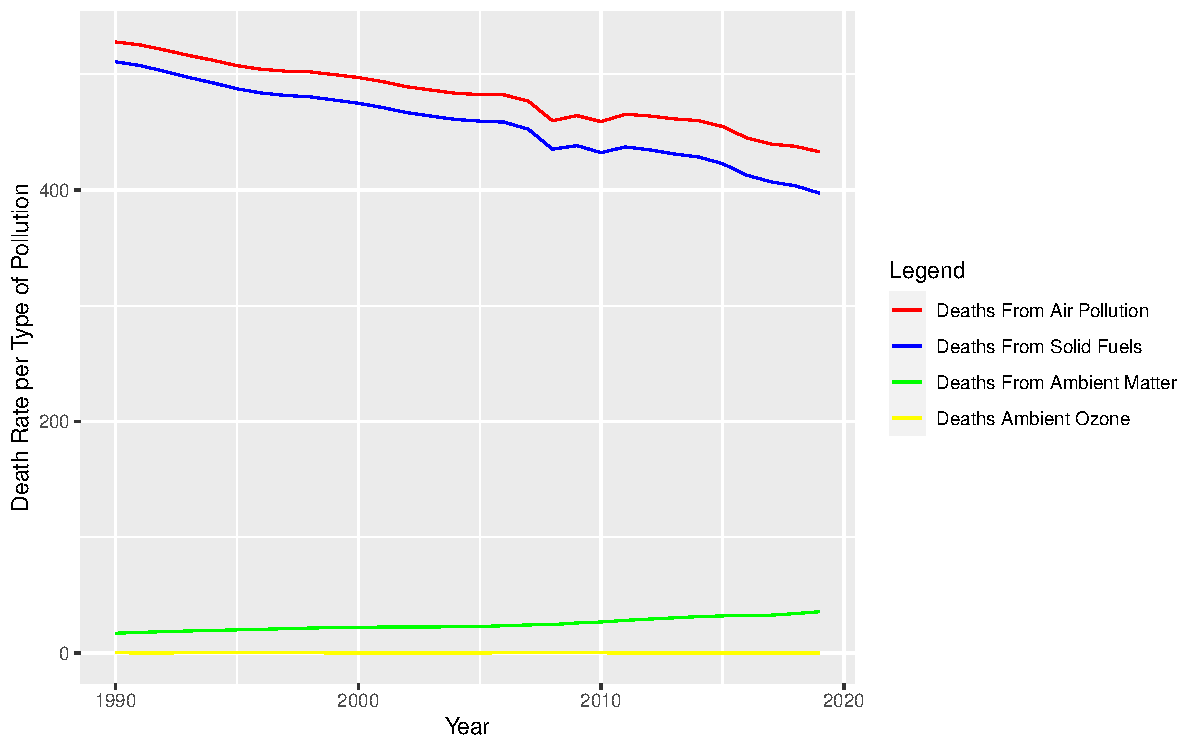
\includegraphics[width=0.8\linewidth]{Assignment4_files/figure-latex/figure1-1} 

}

\caption{Solomon Islands - Annual Trend}\label{fig:figure1}
\end{figure}

Referring to figure\ref{fig:figure1}) above, we can see that, although trends are in the declining movement since the start of 1990, the number of deaths caused by both air pollution and solid fuels are terrifying high comparatively. With these numbers, Solomon Islands is assured to be in the stage of air pollution crisis.

As stated by \textcite{hunt2011policy} in the research paper, health hazards endpoints which quantified are including, but not limited to Premature Mortality, Respiratory and Cardiovascular Illness, Cancer, or even Infant Mortality. Therefore, Solomon Islands living condition is still at an alarming stage which need immediate addressed.

Following this, we are looking at the lowest end for least number of deaths caused by pollution; in which Iceland, New Zealand, Australia, and Puerto Rico hold top spots.

\begin{table}[H]

\caption{\label{tab:table1}Top 4 Countries with lowest Air Pollution Death}
\centering
\begin{tabular}[t]{l|r}
\hline
Country & Deaths\_From\_Air\_Pollution\\
\hline
Iceland & 6.789\\
\hline
New Zealand & 7.073\\
\hline
Australia & 7.428\\
\hline
Puerto Rico & 8.288\\
\hline
\end{tabular}
\end{table}

From table\ref{tab:table1}), we can see that less than 9 persons on average resulted in a fatal incident caused by air pollution.

\begin{table}[H]

\caption{\label{tab:table2}Top 4 Countries with lowest Air Pollution Death from Solid Fuels}
\centering
\begin{tabular}[t]{l|r}
\hline
Country & Deaths\_From\_Solid\_Fuels\\
\hline
Puerto Rico & 0.027\\
\hline
Iceland & 0.076\\
\hline
New Zealand & 0.138\\
\hline
Australia & 0.213\\
\hline
\end{tabular}
\end{table}

Furthermore, comparatively to solid fuels-led death, with even less numbers are shown as a result in table \ref{tab:table2}).

By using Iceland as the main example, according to \textcite{barsotti2020probabilistic}, even though air pollution rate is generally excellent in Iceland, a subtle surge in chemical or pollution such as SO2 is considered as a threat to their ozone and breathing environment. Which they have immediate action to tackle and resolve problem as quick as possible.

Hence, these countries are ensured that rapid response in air pollution issue could make a potential bright further for their countries' air for generations.

\hypertarget{report-conclusion}{%
\subsection{Report Conclusion}\label{report-conclusion}}

In conclusion,

\printbibliography

\end{document}
